%&template
\documentclass{article}
\usepackage{src/template}

\endofdump
\usepackage{minted}

\date{2025 -- 11 -- 23}
\useTemplate[NPA, Exercise=5]
\title{NPA -- Exercise 5}


\begin{document}
\maketitle

    \section{}
    \subsection{}
    \begin{tikzpicture}
        \node (image) at (0,0) {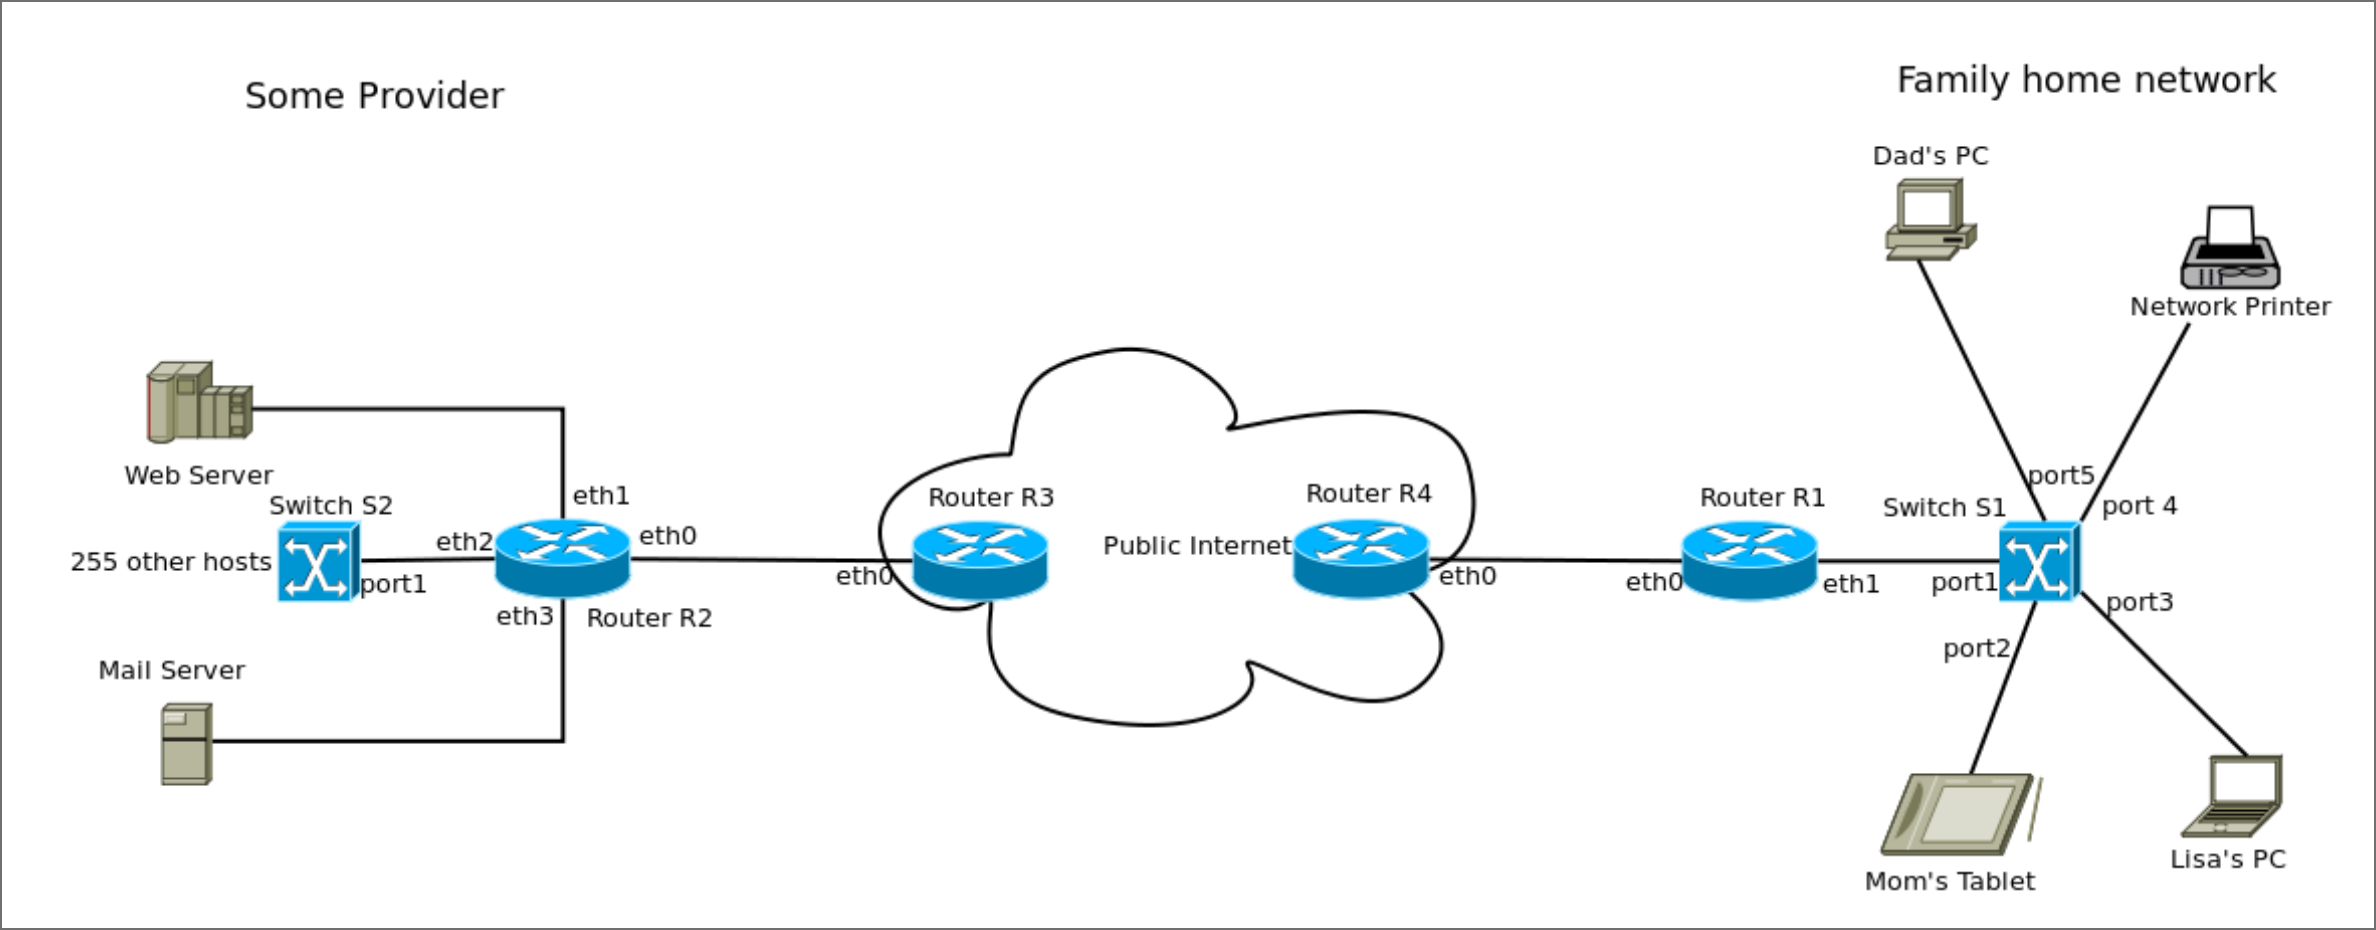
\includegraphics[width=\textwidth]{images/Ex 5a.png}};
        \draw[Orchid, ultra thick] (6.25,0) ellipse (2.1cm and 4.2cm);
        \draw[ForestGreen, ultra thick] (-6.45,-0.7) ellipse (1.7cm and 0.52cm);
        \draw[Orange, ultra thick] (-4.7, -0.4) -- (-4.7, -0.18) -- (-8, -0.18) -- (-8, 1) -- (-4, 1) -- (-4, -0.66);
        \draw[LightSeaGreen, ultra thick] (-4.95, -0.8) -- (-4.95, -1.35) -- (-8, -1.35) -- (-8, -2.5) -- (-4, -2.5) -- (-4, -0.66);

        \draw[blue, ultra thick] (2.7, -0.66) ellipse (1.2cm and 0.5cm);
        \draw[red, ultra thick] (-3, -0.66) ellipse (1.2cm and 0.5cm);
    \end{tikzpicture}

    \subsection{}
    The IP Count is Interfaces + 2. One for the Broadcast and the network address.
    \begin{table}[h]
        \centering
        \begin{tabular}{|l|c|c|}\hline
            Subnet & Number of Interfaces & Number of IPs \\\hline
            \textcolor{Orchid}{Family Home network} & 5 & 7 \\\hline
            \textcolor{Orange}{Some Provider Web} & 2 & 4 \\\hline
            \textcolor{ForestGreen}{Some Provider Switch} & 256 & 258 \\\hline
            \textcolor{LightSeaGreen}{Some Provider Mail} & 2 & 4 \\\hline
            \textcolor{red}{Some Provider Uplink} & 2 & 4 \\\hline
            \textcolor{blue}{Family Home Uplink} & 2 & 4 \\\hline
            
        \end{tabular}
        \caption{Summary of Subnets}
        \label{tab:placeholder}
    \end{table}

    
    
    \section{}
    \subsection{}

    \begin{table}[H]
    \centering
        \begin{tabular}{l l l}
            \textbf{} & \textbf{Network} & \textbf{Example} \\
            \hline
            Linux PCs      & 192.168.0.0/26  & 192.168.0.42/26 \\
            Linux Server   & 192.168.0.64/26 & 192.168.0.84/26 \\
            Windows PCs A  & 192.168.1.0/24  & 192.168.1.42/24 \\
            Windows PCs B  & 192.168.2.0/24  & 192.168.2.42/24 \\
        \end{tabular}
    \end{table}
    
    \subsection{}

    \begin{table}[H]
    \centering
    \begin{tabular}{l r l}
    \textbf{} & \textbf{} & \textbf{Adress} \\
    \hline
    Linux PCs      & Net: & 2001:db8:1000::/64 \\
                   & Example: & 2001:db8:1000::c080:2a/64 \\
                   & Gateway:  & 2001:db8:1000::c080:1/64 \\
    \hline
    Linux Server   & Net: & 2001:db8:1000:1::/64 \\
                   & Example: & 2001:db8:1000:1::c080:54/64 \\
                   & Gateway:  & 2001:db8:1000:1::c080:41/64 \\
    \hline
    Windows PCs A  & Net: & 2001:db8:1000:2::/64 \\
                   & Example: & 2001:db8:1000:2::c080:12a/64 \\
                   & Gateway:  & 2001:db8:1000:2::c080:101/64 \\
    \hline
    Windows PCs B  & Net: & 2001:db8:1000:3::/64 \\
                   & Example: & 2001:db8:1000:3::c080:22a/64 \\
                   & Gateway:  & 2001:db8:1000:3::c080:201/64 \\
    \end{tabular}
    \end{table}
    
    \subsection{}

    \begin{enumerate}[label=(\roman*)]
        \item The NAT router changes the source IP to the single public IPv4 address (its own address) and changes the source port to a yet unused number by the NAT table and stores it.
        \item The NAT router must keep the LAN side IP address and port (source IP and port of the original packet) and the WAN side IP address and port (new source IP and port of the new packet) when its sent out.
    \end{enumerate}

    \subsection{}

    \begin{table}[H]
    \centering
        \begin{tabular}{l l l l}
            \textbf{WAN addr} & \textbf{WAN port} & \textbf{LAN addr} & \textbf{LAN port} \\
            \hline
            133.178.23.14 & 8000 & 192.168.1.2  & 8000 \\
            133.178.23.14 & 8001 & 192.168.1.3  & 8000 \\
            133.178.23.14 & 8002 & 192.168.1.4  & 8000 \\
            133.178.23.14 & 80   & 192.168.0.66 & 80
        \end{tabular}
    \caption{NAT table}
    \label{tab:nat}
    \end{table}
    
    
    \subsection{}

    If an IP packet was sent from 141.42.4.130 to winA002 with internal IP 192.168.1.3, the NAT router would change the destination address (and port if necessary) of the packet from its own external address and port, to the internal IP of winA002 and the respective port of the desired application. 

    Its own external address and port together with the internal address and port of winA002 are saved to the NAT table. 

    
    \newpage
    \subsection{}

    \begin{enumerate}[label=(\roman*)]
        \item 64:ff9b::cb00:7128 (64:ff9b::203.0.113.40)
    
        \item 
        \begin{enumerate}[label=\alph*)]
            \item IPv6 link
    
            \begin{tabular}{>{\ttfamily}l l >{\ttfamily}l l l}
            \hline
            Source IP & Source port & Dest. IP & Dest. port & Protocol \\
            \hline
            2001:db8:1000:2::c080:12a & 5000 & 64:ff9b::cb00:7128 & 443 & TCP \\
            \hline
            \end{tabular}
    
            \vspace{1em} % Abstand zur nächsten Tabelle
    
            \item IPv4 link
    
            \begin{tabular}{>{\ttfamily}l l >{\ttfamily}l l l}
            \hline
            Source IP & Source port & Dest. IP & Dest. port & Protocol \\
            \hline
            133.178.23.14 & 5000 & 203.0.113.40 & 443 & TCP \\
            \hline
            \end{tabular}
    
        \end{enumerate}
    
        \item The NAT64 translates the source IP address and destination IP address. The source port can be changed when necessary, but does not need to be translated in terms of IPv4/IPv6 translation.
    \end{enumerate}



    %# IPv6
    %- 128bit, 8\*16 Bit in hex
    %- hextets separated by :
    %- leading zeros left out
    %- :: for multiple 0 hextets
    %- address split in network part (Subnet prefix) and interface ID
    %NAT64 Address scheme
    %- translate ipv4 to ipv6 using 64:ff9b prefix and ipv4 address as last 32 byte


    
\end{document}https://www.overleaf.com/project/68f8ebe421ecb652f0990b49